il punto critico del sistema � il db e principalmente le op di scrittura 

abbiamo fatto uno script per testare le performance in scrittura e abbiamo cercato di capire come ottimizzare il db per le scritture

tre config di sharding
1 shard
2 shard id
2 shard hashed

parlare del balancer
dei lock di scrittura


come abbiamo eseguito i test:

3 VM 512mb ram, 1,2 ghz
1. mongos+config
2. mongod s1
3. mongod s2

media su 3 run


\begin{table}[h]
\begin{center}
\begin{tabular}{r||r|r|r}
Client & 1 Shard & 2 Shard (id) & 2 Shard (hashed id) \\ 
\hline \hline 
1 & 0.239 & 0.172 & 0.285 \\
10 & 0.451 & 0.442 & 0.448 \\
20 & 0.884 & 0.909 & 0.983 \\
30 & 1.310 & 1.395 & 1.460 \\
40 & 1.776 & 1.859 & 1.960 \\
50 & 2.281 & 2.319 & 2.525 \\
60 & 2.751 & 2.862 & 3.112 \\
70 & 3.275 & 3.484 & 3.925 \\
80 & 3.798 & 3.910 & 4.525 \\
90 & 4.201 & 4.358 & 4.856 \\
100 & 4.784 & 4.967 & 5.604 \\
\end{tabular}
\caption{Tabella small}\label{tab:benchmark-small}
\end{center}
\end{table}

\begin{figure}[h]
\centering
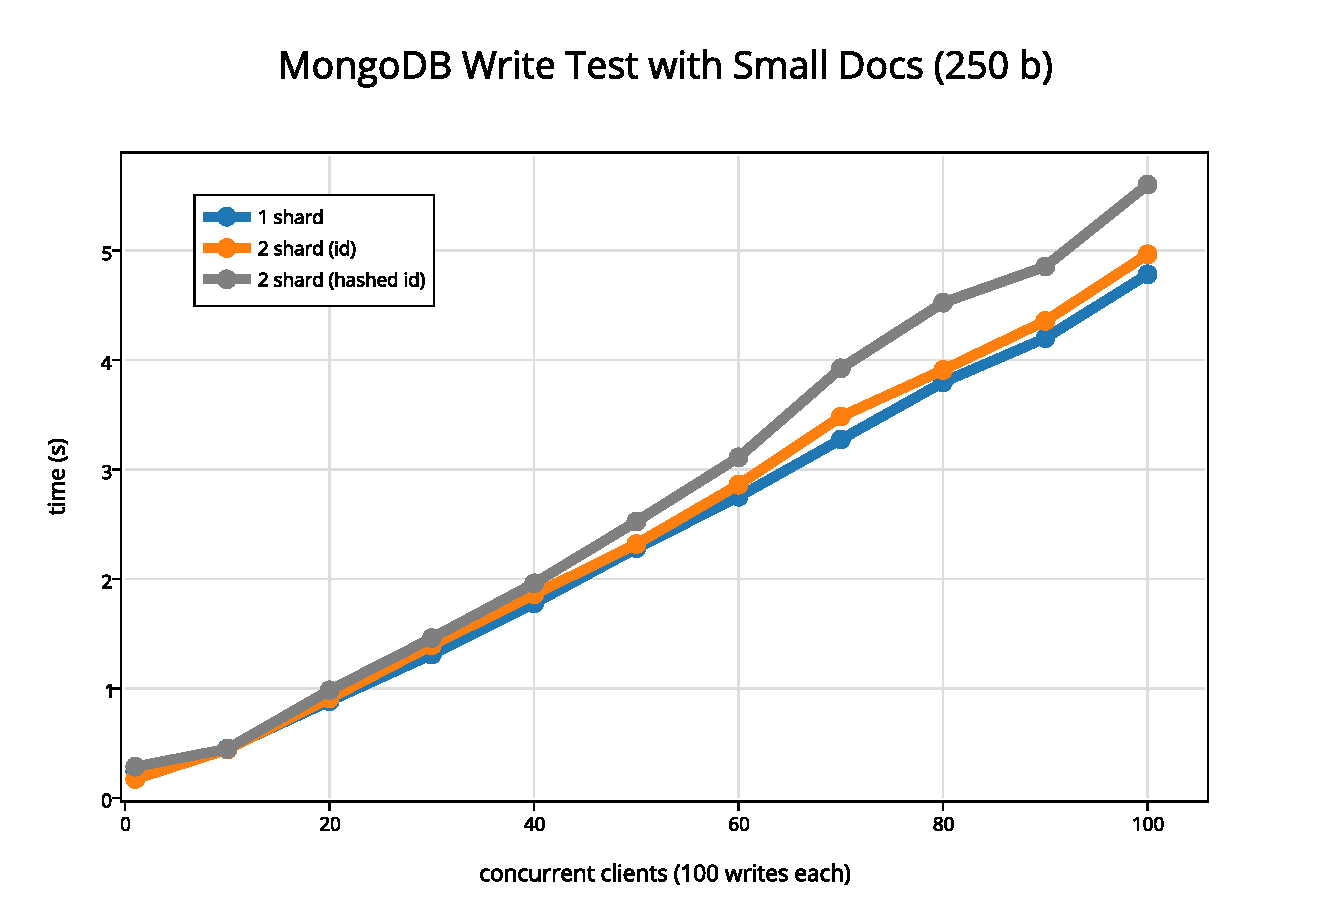
\includegraphics[width=1.0\linewidth]{./img/mongodb_write_test_with_small_docs_250_b}
\caption[small]{small}
\label{fig:benchmark-small}
\end{figure}

\begin{table}[h]
\begin{center}
\begin{tabular}{r||r|r|r}
Client & 1 Shard & 2 Shard (id) & 2 Shard (hashed id) \\ 
\hline \hline 
1 & 0.682 & 0.828 & 0.692 \\
10 & 2.165 & 2.853 & 2.095 \\
20 & 7.009 & 7.243 & 4.290 \\
30 & 8.753 & 10.141 & 6.335 \\
40 & 14.535 & 15.912 & 9.089 \\
50 & 31.931 & 43.645 & 12.949 \\
60 & 30.808 & 24.503 & 15.000 \\
70 & 46.350 & 59.534 & 19.179 \\
80 & 32.045 & 43.703 & 28.898 \\
90 & 114.287 & 97.787 & 25.843 \\
100 & 127.658 & 88.600 & 32.171 \\
\end{tabular}
\caption{Tabella big}\label{tab:benchmark-big}
\end{center}
\end{table}

\begin{figure}[h]
\centering
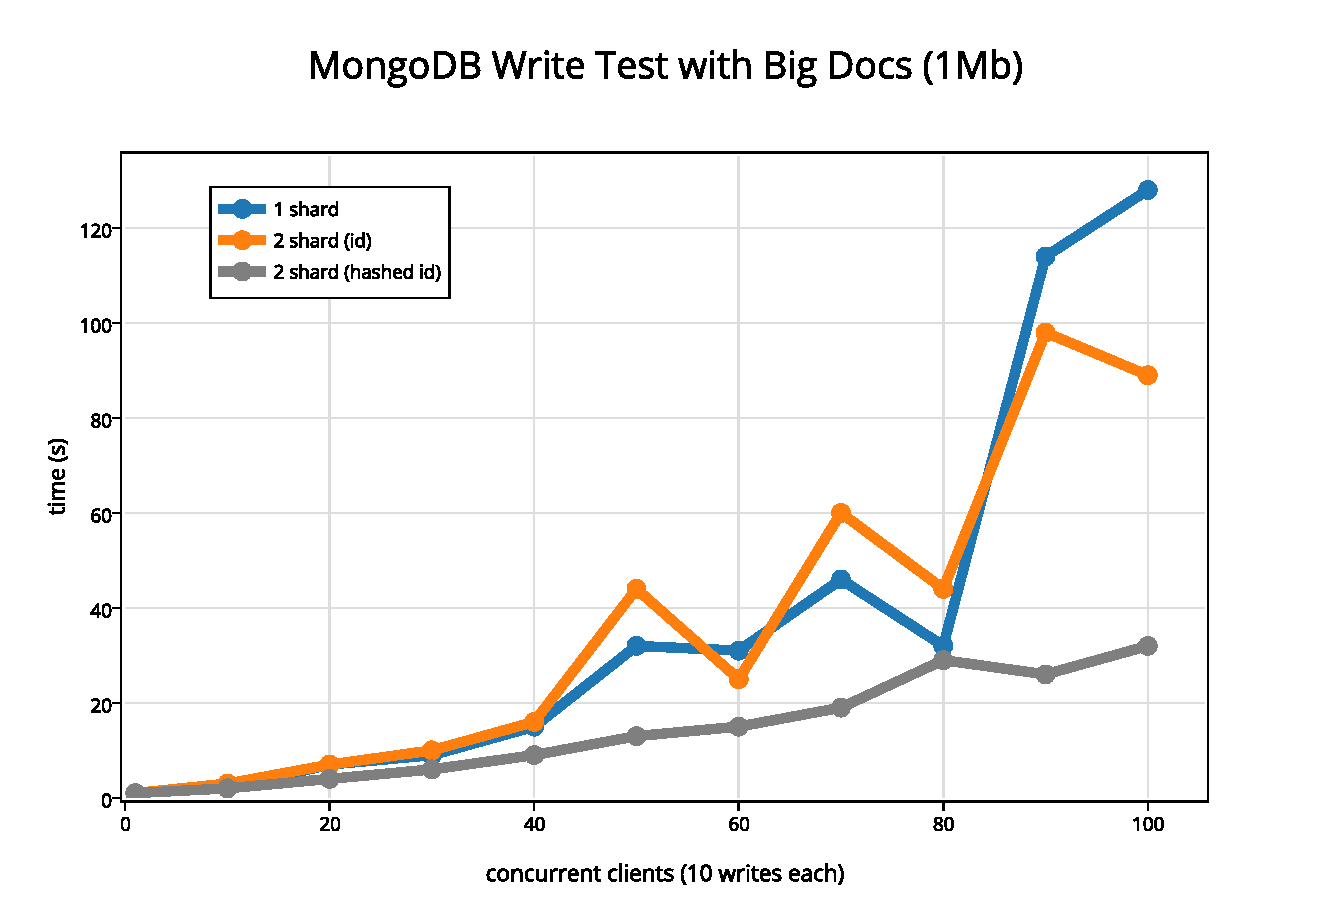
\includegraphics[width=1.0\linewidth]{./img/mongodb_write_test_with_big_docs_1mb}
\caption[big]{big}
\label{fig:benchmark-big}
\end{figure}

%problemi con i benchmark
%- dipendi dalla rete su cui sei
%- nostro client fatto con node - perch� non l'abbiamo usato
%- 2 parole sul tool che abbiamo usato
%- come sono stati fatti i benchmark
%- specifiche del sistema VM, ram, hdd, ...
%- risultati ottenuti


%non ha senso testare mole (server) per la parte rabbit (spiegare)
%il vero collo di bottiglia � il db
%abbiamo testato con configurazioni di db differenti

% parlare dei casini con le chiavi di shard


%conclusioni
%- la coda dei denormalizzatori rompe tra un test e l'altro (coda lunga async)

%problema bench su stessa macchina del server
%    v
%configuraz con vms 
%    v
%bench macchina fisica diversa
%    v
%shard key / ulimit(?)S
%    v





%strano comportamento: no denorm, gli dici di fare 10000 insert e trovi %10499[esatti] doc...
%--> motivo query su sources + insert in whispers #fail mi sa...

%con la nuova chiave lo sharding � sbilanciato 93% / 7%

%i write lock non sembrano avere drammi
%che sia la memoria?


% muore il socket sul benchmark

